\section{Method}
\label{sec:method}

\subsection{Task and Pre-processing}
\label{sec:method:task}

We frame P\&ID digitization as an image-to-graph problem.
Given a raster image $I$, the goal is to recover a process graph
$G = (V, E)$ where each node $v \in V$ carries a bounding box and
a class label from the set \{\textit{valve, pump, instrumentation,
general, tank, arrow, inlet/outlet}\}, and each edge $e \in E$ is
typed as either \textit{solid} or \textit{non-solid}.

\noindent\textbf{Connector collapsing.}
Raw P\&ID annotations from the OPEN100 benchmark include two auxiliary
node types that have no physical counterpart: \emph{connector} nodes
(${\approx}8\times8$~px waypoints that mark pipe bends and junctions)
and \emph{crossing} nodes (where two pipes pass over each other without
connecting). Together these account for 50--65\% of all annotated
nodes. We remove them before training: connector chains are contracted
into direct edges between the physical components at their endpoints,
with the majority edge type along the chain used as the label for
the resulting edge; crossing nodes are simply deleted. This leaves
a graph of physically meaningful components and connections, which
is what an engineer actually cares about.

\subsection{Topology-Preserving Synthetic Generation}
\label{sec:method:generation}

\begin{figure*}[t]
    \centering
    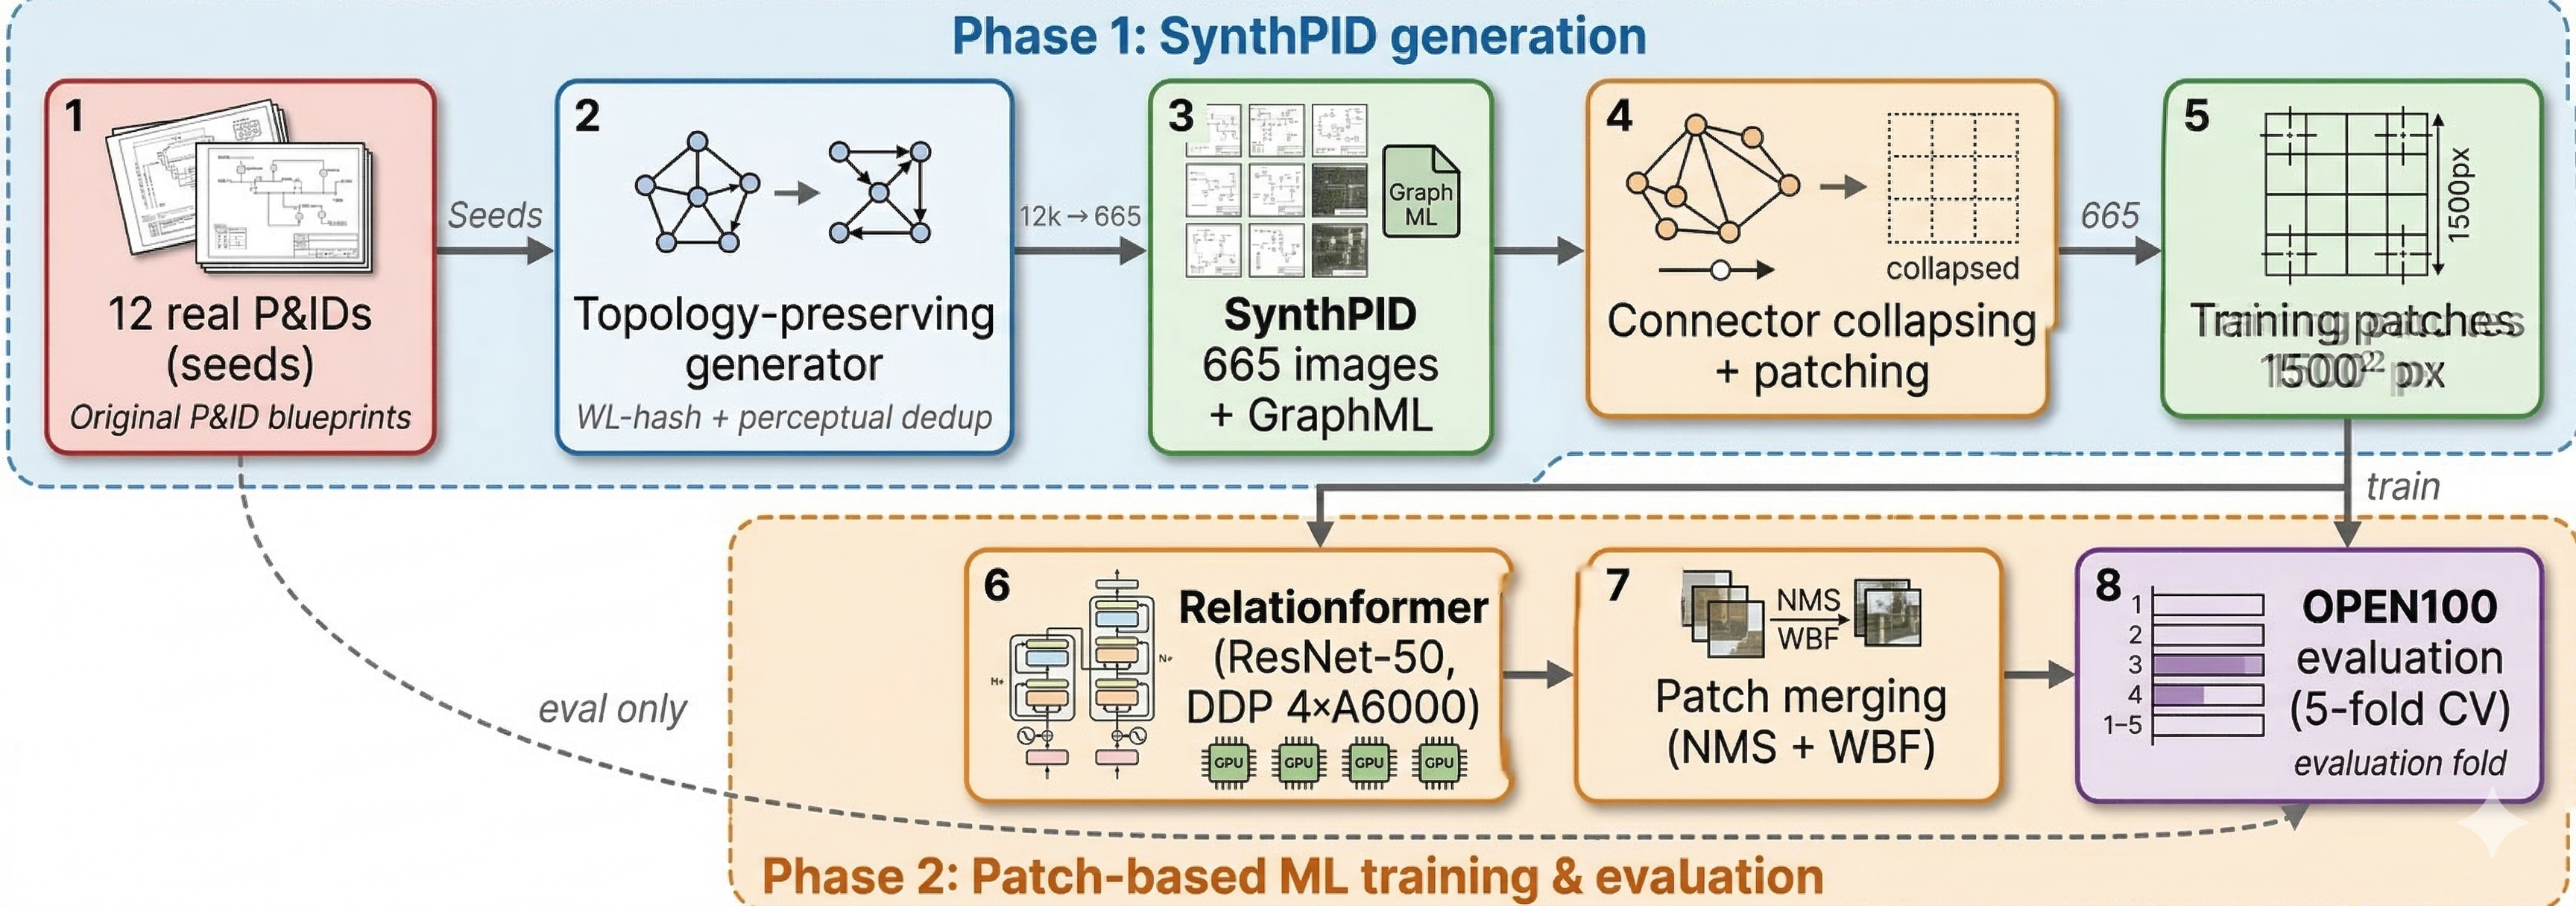
\includegraphics[width=\linewidth]{pipeline_overview_2.jpeg}
    \caption{
        \textbf{Method overview.}
        Twelve real P\&IDs serve as structural seeds. Our generator
        perturbs each seed's topology and re-renders it, producing
        \ours{}: 665 diverse synthetic P\&IDs with full graph
        annotation. After connector collapsing and patch extraction,
        a Relationformer is trained on these patches and evaluated
        on the original real images via patch merging.
    }
    \label{fig:pipeline}
\end{figure*}

\noindent\textbf{Why existing generators fail.}
Template-based methods~\cite{paliwal2021,sturmer2025} place symbols
at random positions and connect them with simple lines.
The graphs this produces have artificially narrow degree distributions
--- most nodes have degree 2 or 3 --- and no spatial clustering that
would reflect, say, an instrument cluster around a vessel or a valve
group on a high-pressure line.
Figure~\ref{fig:dataset_comparison} illustrates the visual gap between
real and synthetic diagrams; Figure~\ref{fig:graph_stats} shows that the
structural gap is at least as large.
A model that has only seen randomly connected graphs will have learned
the wrong priors about which component pairs are likely to be connected,
and this explains the poor transfer performance reported
in~\cite{sturmer2025}.

\noindent\textbf{Generating from seeds.}
Our approach starts from the collapsed graph of a real P\&ID and
generates new images by perturbing it, rather than building from an
empty canvas.
Each generation step proceeds as follows.
First, the collapsed graph $G_s = (V_s, E_s)$ of a seed P\&ID is
extracted.
Node positions are then perturbed within the topological constraints of
the graph: each node is displaced by a small random offset, while its
adjacency is preserved.
Symbols are replaced by randomly sampled templates from the same class,
introducing visual variety without changing component types.
Pipe connections are re-routed using Manhattan routing to reflect the
new positions, and the whole layout is rendered to a high-resolution
PNG with a synchronised GraphML annotation.
A candidate image is accepted only if its Weisfeiler-Lehman
hash~\cite{shervashidze2011} does not match any previously accepted
graph (catching structural duplicates) and its perceptual
hash~\cite{phash} is sufficiently far from all prior images
(catching visual near-duplicates).
Running this process against all 12 seeds over roughly 12,000 total
attempts, we accept \textbf{665 images}, which we name \ours{}.

\begin{figure}[h]
    \centering
    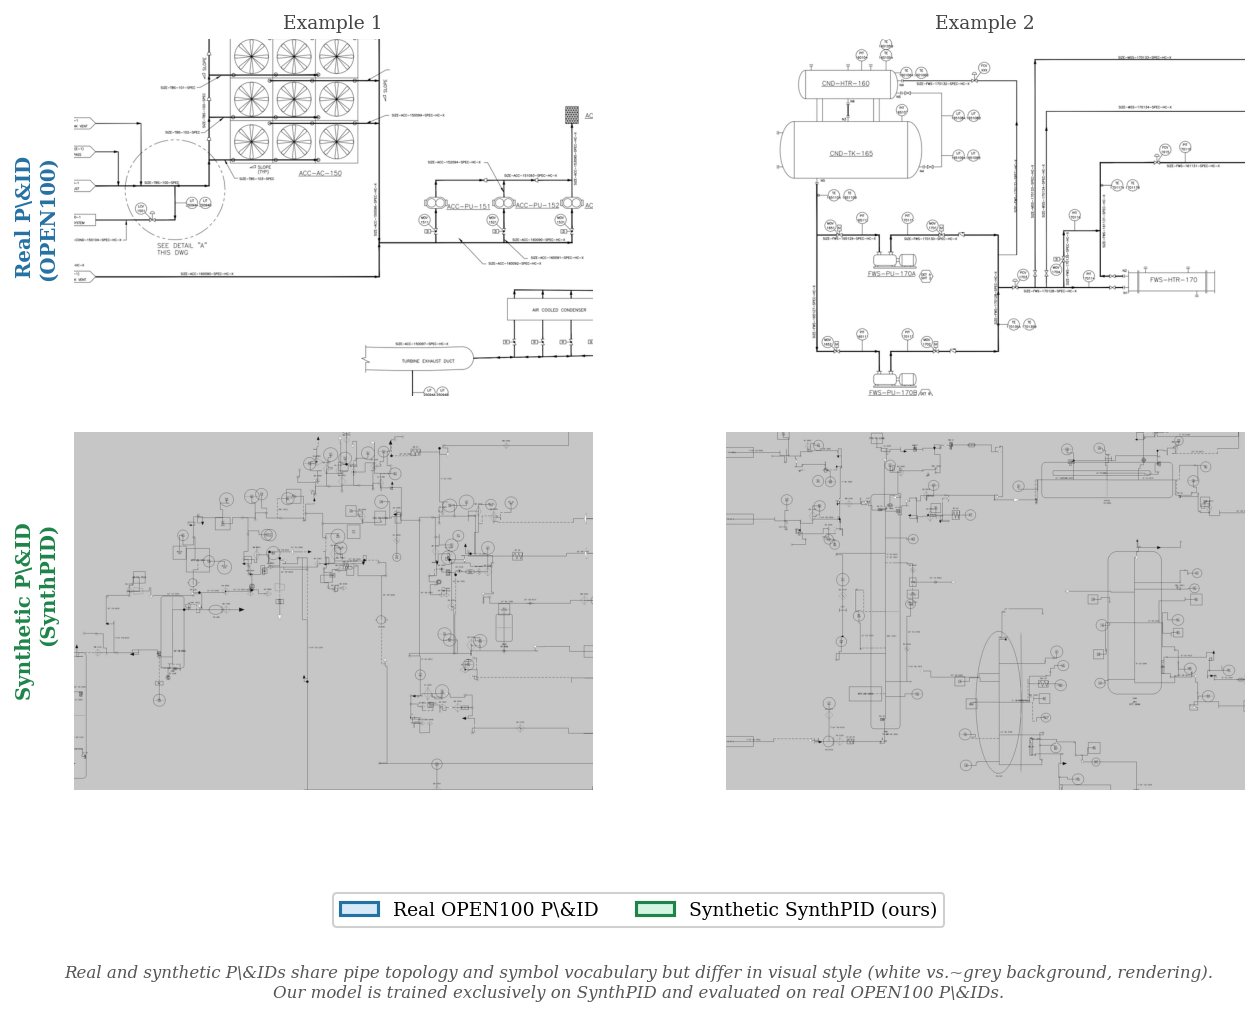
\includegraphics[width=\linewidth]{comparison.png}
    \caption{
        \textbf{The visual domain gap.}
        Real OPEN100 P\&IDs (top) have white backgrounds and
        professional drafting conventions; \ours{} images (bottom)
        have a grey background and a different rendering style.
        Despite this, both share the same symbol vocabulary and,
        critically, the same pipe topology statistics.
    }
    \label{fig:dataset_comparison}
\end{figure}

\noindent\textbf{Structural alignment.}
Figure~\ref{fig:graph_stats} compares degree distributions and
edge densities across real, seed-generated, and template-generated
data.
\ours{} closely matches the real distribution in both respects,
while template-generated diagrams are notably more regular.
We attribute the +30~pp performance gap between these two generation
strategies directly to this structural alignment.

\begin{figure}[h]
    \centering
    
\includegraphics[width=\linewidth]{graph_statistics.png}
    \caption{
        Degree distribution (a) and edge density (b) for three
        corpora. \ours{} tracks the real OPEN100 distribution
        closely; template-based synthetic data does not.
    }
    \label{fig:graph_stats}
\end{figure}

\subsection{Patch-Based Processing}
\label{sec:method:patching}

Full P\&ID images are very large --- typically $7000\times4500$~px
or more --- and the symbols within them are small, often just
$8\times8$~px.
At the image scales required by a DETR-based detector (roughly 800~px
on the long side), symbols shrink to sub-pixel dimensions and box
regression becomes unreliable.
Following~\cite{sturmer2025}, we process P\&IDs by extracting
overlapping $1500\times1500$~px patches at a stride of 750~px,
which brings individual symbols to 50--200~px, a comfortable range
for Deformable DETR.

At patch boundaries, a pipe connection may be cut in two.
We handle this by inserting a \emph{border node} at the intersection
of the connection and the patch edge, so that stitching can later
reconnect the two halves.
After per-patch inference, predictions are merged back into a
full-plan graph in four steps: border confidence attenuation
(partially cropped symbols near the patch edge are down-weighted),
cross-patch duplicate suppression via NMS followed by Weighted Box
Fusion (WBF)~\cite{solovyev2021}, border-node matching to reconnect
cross-boundary edges, and removal of self-loops and isolated nodes.
Both \ours{} and OPEN100 pass through this identical pipeline,
so training and evaluation are processed at the same effective scale.

\subsection{Graph Extraction Model}
\label{sec:method:model}

We use Relationformer~\cite{shit2022} as the detection and relation
prediction backbone.
Relationformer augments Deformable DETR~\cite{zhu2021} with a single
shared \emph{relation token} that is concatenated pairwise with each
object query before the final prediction heads, enabling joint
bounding-box, class, and edge prediction in a single forward pass.
We keep the architecture identical to~\cite{sturmer2025}: ResNet-50
backbone (ImageNet pre-trained), 256-dimensional hidden features,
and 401 object queries per patch.
The P\&ID-specific changes are the output vocabularies ---
7 node classes and 2 edge types (Table~\ref{tab:classes}) --- and
an increased edge loss weight of $\lambda_\text{edge}=5.0$,
which we found beneficial given the difficulty of edge prediction
relative to node localisation.

\begin{table}[h]
\centering
\caption{Output vocabulary used throughout all experiments.}
\label{tab:classes}
\small
\begin{tabular}{ll}
\toprule
\textbf{Node classes (7)} & \textbf{Edge classes (2)} \\
\midrule
valve, pump, instrumentation & solid \\
general, tank, arrow, inlet/outlet & non-solid \\
\bottomrule
\end{tabular}
\end{table}

\subsection{Evaluation Metric}
\label{sec:method:metric}

We adopt the edge mAP metric introduced by~\cite{sturmer2025}
(Algorithm~A1 of that paper) to allow direct numerical comparison.
In brief, predicted and ground-truth nodes are first matched by
bounding-box gIoU using the Hungarian algorithm~\cite{kuhn1955}.
A predicted edge is counted as a true positive only when both
endpoint nodes are correctly matched and the edge type agrees.
Average Precision is then computed from the precision-recall
curve and averaged over the two edge classes.
We additionally report node mAP@0.5~IoU, computed on the full
stitched plan after patch merging.
